\documentclass[10pt]{article}
\usepackage{amsmath}
\usepackage{tikz}
\usepackage{amsfonts}
\usepackage{enumitem}
\usepackage[math-style=ISO,bold-style=ISO,mathrm=sym]{unicode-math}
\usepackage{pdfpages}
\usepackage{tikz}
\usepackage{xcolor}
\usepackage{xfp}
\usepackage[top=5mm, bottom=2mm, inner=5mm, outer=5mm,
headheight=0mm, headsep=0mm, footskip=0mm,
papersize={210mm, 148mm},
includeheadfoot
]{geometry}
\newcommand{\heading}[1]{
\begin{center}
\setmainfont{Raleway SemiBold}[Scale=1.3]#1
\end{center}\vspace{-7mm}}
\newcommand{\subheading}[1]{
\vspace{-2mm}
\begin{flushleft}
\setmainfont{Raleway SemiBold}[Scale=1]#1
\end{flushleft}\vspace{-5mm}}

\defaultfontfeatures{Ligatures=TeX}
\setmainfont[BoldItalicFont=Linux Biolinum Slanted Bold]{Libertinus Sans}
\setmathfont[NFSSFamily=mathfont,RawFeature={+ss08}]{Libertinus Math}
\DeclareMathAlphabet{\mathcal}{OMS}{cmsy}{m}{n}

% Replace 0-9 with sans serif versions
%\DeclareSymbolFont{MathFont}{TU}{mathfont}{m}{n}
\Umathcode "31 = "0"0"1D7E3
\Umathcode "32 = "0"0"1D7E4
\Umathcode "33 = "0"0"1D7E5
\Umathcode "34 = "0"0"1D7E6
\Umathcode "35 = "0"0"1D7E7
\Umathcode "36 = "0"0"1D7E8
\Umathcode "37 = "0"0"1D7E9
\Umathcode "38 = "0"0"1D7EA
\Umathcode "39 = "0"0"1D7EB
\Umathcode "30 = "0"0"1D7E2


\pagestyle{empty}

\newenvironment{enumerlist}[1][5mm]{\begin{enumerate}[leftmargin=#1]
  \setlength{\itemsep}{1pt}
  \setlength{\parskip}{0pt}
}{\end{enumerate}}
\begin{document}
\noindent\begin{minipage}[t][138mm][t]{95mm}
\heading{Definitions}
\vspace{3mm}
{\footnotesize
\begin{enumerlist}[0mm]
\item[] The \textbf{integers} are the numbers \dots, -3, -2, -1, 0, 1, 2, 3, \dots
\item[] The \textbf{positive integers} are the numbers 1, 2, 3, \dots
\end{enumerlist}
}

\vspace{2mm}

\heading{Hints}
\vspace{3mm}
{\footnotesize
\begin{enumerlist}[10mm]
\item[1.] There are only a few odd numbers to add up.
\item[2.] What is the sum of the odd integers between 0 and 2? Between 0 and 4? 0 and 6? What's the pattern?
\item[3.] Try some numbers of baubles between 2 and 20.
\item[4.] What would be the answer for 2 or 3 people? Or 2 or 3 or 4 people? Can you generalise?
\item[5.] It's not too much bigger than 100.
\item[6.] How many one-digit integers? How many two-digit integers? How many three-digit integers? {\dots} What's the most digits the number could have?
\item[7.] If you find four numbers in a row that you can make, you could make all larger scores by adding some 4s.
\item[8.] Try it with a few smaller numbers and look for a pattern.
\item[9.] $10=1+2+3+4$, $11=5+6$, $12=3+4+5$. Keep going until there's one you can't do.
\item[10.] What's special about numbers that are the sum of four consecutive integers?
\item[11.] Try it with 3 points, 4 points, 5 points, and look for a pattern.
\item[12.] Use your pattern from 11.
\end{enumerlist}
}

%\heading{Solutions}
%\vspace{3mm}
%{\footnotesize
%
%}
\vfill
\begin{center}\footnotesize
\includegraphics[width=.14\textwidth]{scorpion.png}
\\
\includegraphics[width=.75\textwidth]{logo.jpg}
\\
\begin{minipage}{3.5cm}
chalkdustmagazine.com
\\
@chalkdustmag
\\
\#ChalkdustChristmasCard2025
\end{minipage}
\end{center}
\end{minipage}\hspace{10mm}\begin{minipage}[t][138mm][t]{95mm}
\vspace*{-1mm}

\begin{center}
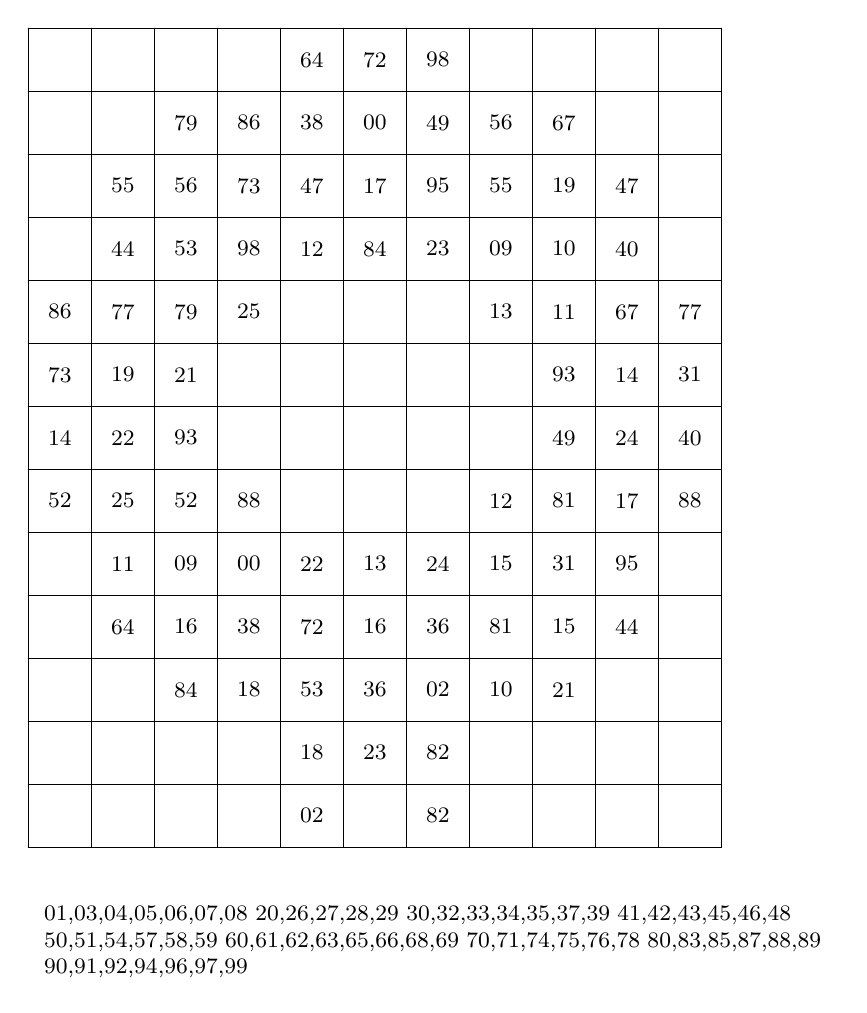
\begin{tikzpicture}[y=8mm,x=8mm,line width=0.5pt,line cap=round,line join=round]
\footnotesize
\begin{scope}[shift={(0.5,0.5)}]
\node[text width=10cm] at (6,-2) {
01,03,04,05,06,07,08
20,26,27,28,29
30,32,33,34,35,37,39
41,42,43,45,46,48
50,51,54,57,58,59
60,61,62,63,65,66,68,69
70,71,74,75,76,78
80,83,85,87,88,89
90,91,92,94,96,97,99
};
\node at (5,2) {36};\node at (6,3) {36};

\node at (8,6) {49};\node at (6,11) {49};
\node at (2,6) {93};\node at (8,7) {93};
\node at (3,3) {38};\node at (4,11) {38};
\node at (8,5) {81};\node at (7,3) {81};
\node at (5,10) {17};\node at (9,5) {17};
\node at (5,12) {72};\node at (4,3) {72};
\node at (3,5) {88};\node at (10,5) {88};
\node at (2,2) {84};\node at (5,9) {84};

\node at (5,4) {13};\node at (7,8) {13};

\node at (3,8) {25};\node at (1,5) {25};
\node at (0,5) {52};\node at (2,5) {52};
\node at (2,7) {21};\node at (8,2) {21};

\node at (7,5) {12};\node at (4,9) {12};
\node at (5,1) {23};\node at (6,9) {23};

\node at (6,12) {98};\node at (3,9) {98};
\node at (0,8) {86};\node at (3,11) {86};
\node at (4,12) {64};\node at (1,3) {64};
\node at (10,6) {40};\node at (9,9) {40};
\node at (7,9) {09};\node at (2,4) {09};

\node at (1,4) {11};\node at (8,8) {11};

\node at (9,7) {14};\node at (0,6) {14};
\node at (9,3) {44};\node at (1,9) {44};
\node at (4,10) {47};\node at (9,10) {47};
\node at (3,10) {73};\node at (0,7) {73};
\node at (8,4) {31};\node at (10,7) {31};
\node at (1,7) {19};\node at (8,10) {19};
\node at (9,4) {95};\node at (6,10) {95};
\node at (7,10) {55};\node at (1,10) {55};
\node at (2,10) {56};\node at (7,11) {56};
\node at (9,8) {67};\node at (8,11) {67};
\node at (1,8) {77};\node at (10,8) {77};
\node at (2,8) {79};\node at (2,11) {79};

%%%%%%%%%%%%%%%% RED %%%%%%%%%%%%%%%%%%%

\node at (2,3) {16};\node at (5,3) {16};

\node at (7,2) {10};\node at (8,9) {10};
\node at (3,4) {00};\node at (5,11) {00};
\node at (6,2) {02};\node at (4,0) {02};

\node at (8,3) {15};\node at (7,4) {15};
\node at (2,9) {53};\node at (4,2) {53};

\node at (3,2) {18};\node at (4,1) {18};
\node at (6,0) {82};\node at (6,1) {82};
\node at (4,4) {22};\node at (1,6) {22};
\node at (6,4) {24};\node at (9,6) {24};

\end{scope}



%\foreach \x/\y in {
%    5/1,
%    2/2,5/2,8/2,
%    1/3,3/3,4/3,6/3,7/3,9/3,
%    1/4,2/4,5/4,8/4,9/4,
%    0/5,1/5,2/5,3/5,7/5,8/5,9/5,10/5,
%    0/6,2/6,8/6,10/6,
%    0/7,1/7,2/7,8/7,9/7,10/7,
%    0/8,1/8,2/8,3/8,7/8,8/8,9/8,10/8,
%    1/9,3/9,4/9,5/9,6/9,7/9,9/9,
%    1/10,2/10,3/10,4/10,5/10,6/10,7/10,8/10,9/10,
%    2/11,3/11,4/11,6/11,7/11,8/11,
%    4/12,5/12,6/12
%}
%    \fill[green] (\x,\y) rectangle +(1,1);
%\foreach \x/\y in {
%    4/0,6/0,
%    4/1,6/1,
%    3/2,4/2,6/2,7/2,
%    2/3,5/3,8/3,
%    3/4,4/4,6/4,7/4,
%    1/6,9/6,
%    2/9,8/9,
%    5/11
%}
%    \fill[red] (\x,\y) rectangle +(1,1);

\foreach \x in {0,...,11}
    \draw (\x,0) -- +(0,13);
\foreach \y in {0,...,13}
    \draw (0,\y) -- +(11,0);

\end{tikzpicture}

\end{center}

\vfill
\begin{center}
{\setmainfont[Scale=3]{Pacifico}Merry Christmas}\\
{(instructions inside)}
\end{center}
\vfill\null
\end{minipage}

\newpage

\noindent\begin{minipage}[t][138mm][t]{95mm}
\heading{Instructions}
\vspace{3mm}
{\footnotesize
\begin{enumerlist}
\item Solve the puzzles below.
\item For every pair of digits that appears in each answer, colour the two squares on the front
    cover that contain the pair. For example, if an answer in the green section was
    3305, you would colour the squares containing 33, 30 and 05 green.
\end{enumerlist}}

\vspace{-1mm}

\heading{Puzzles}
{\footnotesize
\begin{center}\footnotesize(see back of card for definitions and hints)\end{center}

\vspace{-4mm}
%1. 36
%2. 493817284
%3. 13
%4. 2521
%5. 123
%6. 986409
%7. 11
%8. 1447319556779

%9. 16
%10. 1002
%11. 153
%12. 18224
\subheading{Green}
\begin{enumerlist}
\item[1.] What is the sum of all the odd integers between 0 and 12?
\item[2.] What is the sum of all the odd integers between 0 and 44444?
\item[3.] Carol has more than one bauble.
    When she shares them equally between 3 people, there is one bauble left over.
    When she shares them equally between 4 people, there is still one bauble left over.
    What is the smallest number of baubles that Carol could have?
\item[4.] Carol has more than one bauble.
    When she shares them equally between 2, 3, 4, 5, 6, 7, 8, or 9 people, there is one bauble left over.
    What is the smallest number of baubles that Carol could have?
\item[5.] What is the smallest three-digit positive integer whose digits are all non-zero and different?
\item[6.] How many positive integers are there whose digits are all non-zero and different?
\item[7.] In a Christmas game, you can win either 4 points or 5 points on your turn,
    and the game can last any number of turns. What is the largest number of points that it is impossible to end the game on?
\item[8.] In a different Christmas game, you can win either 495371 points or 2921695 points on your turn,
    and the game can last any number of turns. What is the largest number of points that it is impossible to end the game on?
\end{enumerlist}

\vspace{-1mm}

%
\subheading{Red or yellow}
\begin{enumerlist}
\item[9.] 
What is the smallest two-digit positive integer that cannot be written as the sum of consecutive integers?
\item[10.] What is the smallest four-digit positive integer that can be written as the sum of exactly four consecutive integers?
\item[11.] Holly drew 18 points on the circumference of a circle then drew straight lines connecting
    each pair of points. How many straight lines did she draw?
\item[12.] Holly drew some points on the circumference of a circle then drew straight lines connecting
    each pair of points. She drew 166047976 straight lines. How many points did she draw?
\end{enumerlist}
}
\end{minipage}\hspace{10mm}\begin{minipage}[t][138mm][t]{95mm}
\vfill
\begin{center}
{\setmainfont[Scale=3]{Pacifico}Merry Christmas}\\
\end{center}
\vfill
\begin{center}
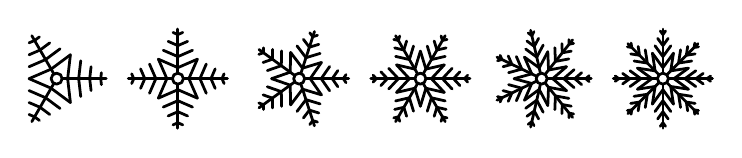
\begin{tikzpicture}[x=7mm,y=7mm,line cap=round,line join=round,line width=1pt]
\foreach \n in {3,...,8} {
\begin{scope}[shift={(2.2*\n,0)}]
\draw (0,0) circle (0.1);
\foreach \i in {1,...,\n} {
    \begin{scope}[rotate=360*\i/\n]
        \draw (0.1,0) -- (0.9,0);

        \foreach \a in {1, 2, 3, 4}
        \draw
            (0.2*\a,0) -- +({(5/4-\a/4)*(0.5*cos(180/\n)-0.2)},{(5/4-\a/4)*0.5*sin(180/\n)})
            (0.2*\a,0) -- +({(5/4-\a/4)*(0.5*cos(180/\n)-0.2)},{-(5/4-\a/4)*0.5*sin(180/\n)});
        %\foreach \a in {1, 2, 3, 4}
        %\draw
        %    (0.03+0.15*\a,0) -- +({0.05*(5-\a)},{0.05*(5-\a)})
        %    (0.03+0.15*\a,0) -- +({0.05*(5-\a)},{-0.05*(5-\a)});
    \end{scope}

}
\end{scope}
}
\end{tikzpicture}
\end{center}
\vspace{1mm}
\end{minipage}


\end{document}

